\chapter{Progettazione e codifica del progetto}\label{cap:progettazione-codifica}

\intro{In questa sezione, saranno elencate le tecnologie principali utilizzate durante lo sviluppo del sistema oggetto del tirocinio.
Inoltre, verrà descritto il ciclo di vita del software, le fasi di progettazione e codifica e le scelte architetturali realizzate, 
a livello di sistema e design pattern.}

\section{Componenti principali del sistema}\label{sec:componenti-principali}
Il sistema risulta essere composto da due parti principali: 
\begin{itemize}
    \item{\textbf{Front-end}}: è la parte visibile all'utente, che permette di interagire con il sistema. È stata sviluppata utilizzando il framework React e il linguaggio TypeScript. 
    Questa comprende la parte grafica da me realizzata e la relativa interazione con il contratto fornito come libreria dallo studente Alessio De Biasi.
    \item {\textbf{Back-end}}: è la parte che gestisce la logica dell'applicazione, che permette di interagire con la blockchain e di gestire le funzionalità del sistema. È stata sviluppata utilizzando il linguaggio Solidity.
    Quest'ultima comprende il contratto sviluppato dallo studente magistrale Alessio De Biasi basato sugli standard \glsfirstoccur{\gls{w3cg}} \glsfirstoccur{\gls{ssig}} e \glsfirstoccur{\gls{didg}}.
\end{itemize}

\section{Tecnologie utilizzate}\label{sec:tecnologie-strumenti}

\subsection{Codifica front-end}

\subsubsection{React}
React è una libreria JavaScript utilizzata per la creazione di interfacce utente. È stata sviluppata da Facebook e rilasciata nel 2013. 
Essa consente di creare dei componenti riutilizzabili che rappresentano parti dell'interfaccia e gestire lo stato dell'applicazione in modo efficiente e scalabile.
Questo lo rende adatto allo sviluppo di applicazioni complesse e dinamiche (specifiche e riferimenti a \cite{site:react}).
Nel mio caso, è utilizzato per la progettazione delle componenti e delle pagine.

\subsubsection{TypeScript}
TypeScript è un linguaggio di programmazione open source sviluppato da Microsoft. È un super-set di JavaScript che aggiunge tipi statici opzionali al linguaggio,
permettendo di scrivere codice più robusto e manutenibile, grazie alla possibilità di definire interfacce e classi (secondo \cite{site:react}).
All'interno delle pagine realizzate, sono stati creati dei tipi appositi per poter gestire più facilmente le informazioni e le funzionalità del sistema.

\subsection{Codifica back-end}

\subsubsection{Solidity}
Solidity è un linguaggio di programmazione orientato agli oggetti per la scrittura di smart contract. È stato sviluppato da Ethereum e permette di gestire
lo stato di un contratto, definire funzioni e interagire con altri contratti all'interno delle blockchain,
grazie alla gestione del sistema di transazioni basato sugli eventi e alla possibilità di definire interfacce (in base a quanto presente in \cite{site:solidity}).
L'interazione con la blockchain e il contratto da richiamare come libreria è stato scritto in questo linguaggio.

\subsection{Librerie di terze parti}

\subsubsection{Node.js}
Node.js è un ambiente di runtime open source per l'esecuzione di codice JavaScript lato server. È basato sul motore JavaScript V8 di Google Chrome e permette di gestire
le dipendenze dell'applicazione, grazie al suo package manager \textit{npm}, differenziando le librerie dell'applicazione e quelle di terze parti.
Tramite semplici comandi, è possibile installare e rimuovere le dipendenze, aggiornarle e gestire le versioni. 
Lo strumento ha permesso una facile configurazione delle dipendenze e la gestione delle versioni (riferimenti in \cite{site:node}).

\subsubsection{web3.js}
web3.js è una collezione di librerie JavaScript per poter interagire facilmente con le blockchain, in particolare con Ethereum.
Essa permette di connettersi ad un nodo della blockchain, inviare transazioni e interagire con gli smart contract, gestendo facilmente il collegamento
e l'interazione tra la parte grafica e gli smart contract, definendo modularmente le funzionalità presenti (\cite{site:web3}).
Grazie a questo, è stato possibile gestire facilmente l'interazione con la blockchain e gli smart contract, permettendo la chiamata al contratto
e alle sue funzioni.

\subsubsection{Hardhat}
Hardhat è un ambiente di sviluppo per le blockchain che permette di testare e distribuire smart contract. Esso permette di distribuire facilmente
in locale per poter testare le funzionalità degli smart contract, e di distribuirli su una blockchain pubblica, come ad esempio
Ethereum (in base alle definizioni e guide in \cite{site:hardhat}).

\subsection{Versionamento}

\subsubsection{GitHub}
GitHub è una piattaforma di hosting per progetti software. Essa permette di gestire il versionamento del codice tramite il sistema di controllo di versione Git.
In particolare, consente lo sviluppo di codice attraverso un \textit{repository} remoto, che permette di gestire le modifiche e le versioni del codice, tenendo traccia attraverso un registro
delle modifiche effettuate e permettendo di tornare ad una versione precedente del codice (\cite{site:github}). 

\subsection{Verifica}

\subsubsection{ESLint}
ESLint è uno strumento di analisi statica del codice per identificare i modelli problematici trovati nel codice \textit{JavaScript} e \textit{TypeScript}.
È stato utilizzato per garantire la qualità del codice prodotto, tramite la definizione di regole e la segnalazione di eventuali errori.

\subsubsection{Jest}
Jest è un framework di test per \textit{JavaScript} e \textit{TypeScript}. È stato utilizzato per la definizione di test unitari e di integrazione, per verificare il corretto funzionamento
delle funzionalità implementate tra le pagine ed i componenti.

\section{Configurazione ambiente di sviluppo}\label{sec:configurazione-ambiente}

\subsection{Smart Contract}
All'interno del mio progetto di stage, per realizzare l'implementazione degli smart contract, ho utilizzato un ambiente di sviluppo locale,
basato su \textit{Hardhat}, un ambiente di sviluppo per Ethereum che permette di testare e distribuire smart contract.
Lo strumento permette la creazione di un ambiente di test locale, sulla base dell'impostazione fornita da specifici \textit{script}, in
grado di gestire la compilazione e la successiva esecuzione (\textit{deploy}) del contratto fornito sulla rete locale.
Per poter effettuare le singole chiamate, lo strumento fornisce un insieme di account di test con un saldo iniziale di 10000 ETH (valute della rete Ethereum, rete \gls{blockchaing} utilizzata dallo strumento), 
che possono essere utilizzati per effettuare le chiamate desiderate qualora siano presenti transazioni (normalmente in esecuzione sulla porta 8545 all'interno della rete locale). \\

Nello specifico, la strutturazione prevede:
\begin{itemize}
    \item uno script di \textit{deploy}, scritto in TypeScript, che definisce il contratto che viene chiamato, il suo indirizzo sulla rete locale
    e la generazione di un file \textit{json} chiamato \textit{ABI}, che contiene le informazioni in formato binario del contratto. Esso viene utilizzato nella parte frontend;
    \item uno script di test, scritto in TypeScript, che permette di testare le funzionalità del contratto, tramite l'ausilio di \textit{web3.js};
    \item uno script di configurazione, che definisce l'account utilizzato sulla rete locale e le librerie presenti.
\end{itemize}

\subsection{Frontend}
Per lo sviluppo del front-end, ho utilizzato un ambiente di sviluppo locale, basato su \textit{Node.js}, un ambiente di runtime per JavaScript.
Tramite questo, è stato possibile gestire le dipendenze del progetto, tramite il package manager \textit{npm}, e avviare un server locale per poter testare
e scrivere le pagine presenti. In particolare, il server è stato avviato sulla porta 3000, per poter permettere l'interazione con il contratto tramite
le funzionalità del front-end e le chiamate al contratto.
Nello specifico, la strutturazione prevede:
\begin{itemize}
    \item una cartella \textit{src}, contenente i file \textit{.js} e \textit{.ts} che definiscono le funzionalità del front-end;
    \item una cartella \textit{public}, contenente i file \textit{.html} e \textit{.css} che definiscono le pagine del front-end;
    \item una cartella \textit{build}, contenente i file \textit{.js} e \textit{.ts} compilati, che vengono utilizzati per l'esecuzione del front-end;
    \item una cartella \textit{node\_modules}, contenente le dipendenze del progetto.
\end{itemize}

\newpage
\section{Progettazione}\label{sec:progettazione-requisiti}

\subsection{Architettura e pattern front-end}

L'utilizzo di React ha permesso di definire una struttura modulare per il front-end, in modo da poter definire facilmente le pagine e le funzionalità.
Esso è formato da un insieme di componenti, che definiscono un insieme di funzioni riutilizzabili, ognuna delle quali definisce un suo comportamento. 
La logica dell'applicazione permette di gestire singolarmente le funzionalità del codice, definendo le pagine come funzioni che vengono
esportate e utilizzate come entità indipendenti. In questo modo, si incrementa la modularità del codice e la sua manutenibilità, in quanto ogni componente
o pagina può essere riutilizzato in modo semplice e può essere modificato senza influenzare il resto del codice. \\

La struttura della pagine è stata definita tramite \textit{.tsx}, un'estensione di \textit{React} che permette di definire la struttura della pagina 
sfruttando elementi strutturali \textit{HTML}, la presentazione con \textit{CSS} e il linguaggio di programmazione \textit{TypeScript} per la gestione della logica, dei tipi e delle variabili.
Tramite l'utilizzo dei cosiddetti \textit{hook}, è stato possibile definire le funzionalità del front-end, in modo da poter gestire le chiamate tra le componenti della 
pagina in base all'attivazione di specifici eventi in modo dinamico, grazie all'uso degli \textit{state}.
In questo modo, i singoli componenti e le pagine, definite come \textit{views}, riescono ad avere singola responsabilità e ne permette un miglior riutilizzo. \\

La logica viene mantenuta separata dalla presentazione, utilizzando la strutturazione a componenti in grado di comunicare nativamente con il 
\textit{DOM (Document Object Model)} della pagina ma aggiungendo la gestione degli eventi in modo nativo tramite React, permettendo così di poter gestire le interazioni con l'utente
solo tramite le componenti e le pagine stesse, separando il codice della pagina dalla sua presentazione realizzata con \textit{CSS}. \\

Dato che React è una libreria grafica, non viene forzato alcun preciso pattern architetturale, ma viene lasciata libertà di scelta allo sviluppatore.
In questo caso, il pattern utilizzato è il \textit{Flux Pattern}, che permette di definire un flusso unidirezionale dei dati, in modo da poter gestire
le interazioni dell'utente con la pagina e le chiamate al contratto in modo semplice e senza dover gestire la sincronizzazione dei dati tra le varie componenti.
Ciò permette all'applicazione di essere gestita da funzionalità precise a cascata, andando ad interagire con l'esterno con semplici aggiunte di moduli o dipendenze.
Come visibile dalla figura \ref{fig:react}, la logica si compone di un componente radice che descrive l'applicazione,
a sua volta costituita eventualmente da uno o più componenti, innestati a vari livelli secondo la relazione di composizione,
includendo anche eventuali componenti di terze parti per permettere la gestione e l'interazione all'esterno, esportando la funzionalità realizzata dal componente
o dalla pagina modularmente. \\

\begin{figure}[h]
    \centering
    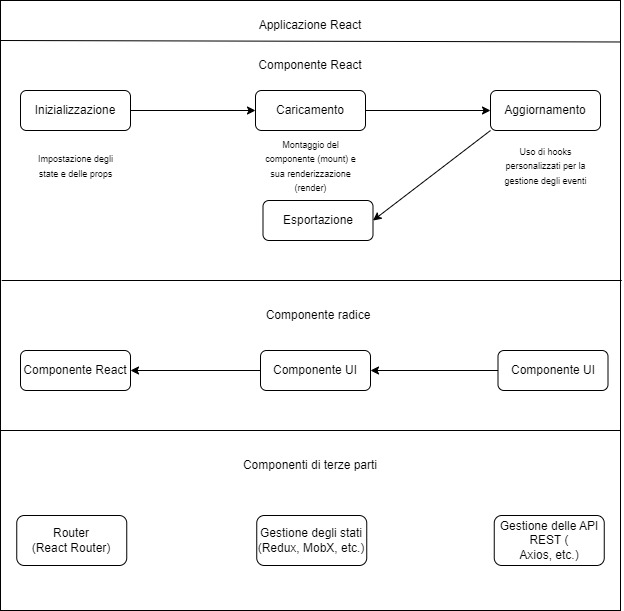
\includegraphics[width=0.6\textwidth, alt={Descrizione dello schema logico di un'applicazione React}]{immagini/react.jpeg}
    \caption{Schema logico applicazione React} \label{fig:react}
\end{figure}


Secondo le \textit{best practices} di React, sono stati utilizzati un insieme di \textit{design pattern} per normare la codifica tipici della libreria grafica:
è stato utilizzato il pattern \textit{Functional Component}, che permette di definire proprietà specifiche (definite come \textit{props})
ed uno stato interno in grado interagire ad eventi asincroni generati da azioni compiute dall'utente nelle varie condizioni definite. La strutturazione si compone di un insieme di funzioni e stati definiti
al caricamento della pagina (utilizzando l'\textit{Hook Pattern}, attraverso gli \textit{hooks} \textit{useEffect} e \textit{useState}), in grado di caricare e gestire dinamicamente le informazioni
al suo interno, esportando poi il componente funzionale o la stessa pagina, secondo un insieme di funzionalità definite dallo specifico contesto. 
Le componenti stesse supportano nativamente il cambiamento dei propri stati tramite la definizione di funzioni di \textit{callback}, eseguendo le funzioni definite al cambiamento di stato,
osservando le azioni dell'utente (definito come \textit{Controlled Components} nel contesto React) secondo il noto pattern \textit{Observer} alle chiamate definite dagli eventi stessi. \\
\\

\newpage
Nello specifico, l'applicazione definisce per ogni pagina una cartella comprensiva del componente funzionale
esportato e del suo stile, e un file di test per verificare le principali funzionalità previste.
La suddivisione delle cartelle individuata riflette la divisione delle responsabilità; di massima, è presente una cartella \textit{components}, contenente i componenti utilizzati da tutte le pagine 
comprensive della barra di navigazione, del \textit{footer} e di eventuali componenti di terze parti, una cartella \textit{views} con le pagine realizzate per l'applicazione ed
una cartella \textit{utils}, con l'insieme delle funzionalità definite all'avvio dell'applicazione e centrali per la comunicazione con blockchain. \\
L'autenticazione viene gestita tramite un contesto, definito dal \textit{Provider Pattern} di React, che permette di definire un contesto globale
in cui tutta l'applicazione e le sue componenti vengono racchiuse per poter accedere alle informazioni definite al suo interno in ogni momento.
Le singole opzioni visibili tra utente autenticato e non autenticato sono invece gestite secondo il pattern \textit{Conditional Rendering}, in grado di differenziare le opzioni
visibili in base al suo stato.

\subsection{Architettura e pattern back-end}
Lo \textit{smart contract} da me utilizzato come libreria per la gestione delle funzionalità di base è stato realizzato in \textit{Solidity}, un linguaggio di programmazione
orientato agli oggetti per la definizione di \textit{smart contract} per la piattaforma \textit{Ethereum}. 
Il contratto è stato creato secondo il pattern \textit{Factory}, che permette di definire un contratto principale, in grado di creare e gestire altri contratti secondari,
ciascuno responsabile della creazione di un'istanza dei documenti di identità con \glsfirstoccur{\gls{didg}} con relativi attributi ed operazioni associate.
Inoltre, per permettere ai singoli componenti di interagire con il contratto, è stato utilizzato il pattern \textit{Singleton}, che assicura la creazione dell'unica istanza
del contratto, in grado di essere utilizzata da tutte le componenti dell'applicazione. \\

L'interazione tra il contratto e la parte frontend si basa sull'interazione nativa e la gestione delle chiamate generate dallo \textit{smart contract} tramite l'utilizzo
della libreria \textit{Node.js}, in grado di gestire le chiamate asincrone e la comunicazione con il contratto stesso tramite ascolto da parte dei componenti e delle pagine
presenti nel front-end dell'applicazione, secondo il pattern \textit{Observer}. 
In questo modo, secondo l'architettura a componenti definita come flusso, è possibile separare completamente la logica di interazione con il contratto dalla logica di visualizzazione,
utilizzando le funzionalità definite con la creazione di una sola riga di codice ed effettuando le chiamate alle funzionalità previste nella parte di codifica 
solamente quando necessario, permettendo la relativa sincronizzazione dei componenti che, ascoltando, aggiornano i propri stati secondo le chiamate effettuate. \\

\textit{Hardhat}, in grado di creare una locale di test, agisce quindi da \textit{middleware} tra la parte front-end e la blockchain, permettendo di simulare le chiamate al contratto
ed ugualmente all'utente di interagire con l'applicazione, senza dover effettivamente effettuare le transazioni sulla rete principale.
Per semplicità di implementazione, le chiamate sono effettuate sulla rete locale con l'utilizzo di profili di test già esistenti, in grado di effettuare le transazioni (ad ogni chiamata
corrisponde una spesa in termini di valuta, coperta completamente dai profili di test). \\

Si consideri che l'applicazione simula il funzionamento della blockchain \textit{Ethereum}, per la quale la descrizione di un'architettura viene
descritta secondo il modello \textit{client-server}, in cui il client è rappresentato dal nodo che effettua la richiesta e il server dal nodo che la riceve e la processa.
Il modello definito come \textit{Dapp architecture}, descrive complessivamente l'interazione adottata nel progetto, come visibile da figura \ref{fig:eth-architecture}.
\begin{itemize}
\item l'utilizzo di una base di dati locale nel quale vengono salvati i dati relativi all'utente, in grado di essere utilizzati per l'autenticazione e per la creazione dei documenti di identità.
Nel caso del progetto, ogni dato viene salvato in locale all'interno di \textit{localStorage}, successivamente cifrata localmente secondo quanto sarà descritto in sezioni di codifica e 
poi effettuando le chiamate al contratto per la creazione dei documenti di identità tramite le chiamate del server presente;
\item l'utilizzo del codice per memorizzare le transazioni, che permette di considerare uno smart contract, compilarlo e inserire il suo \textit{bytecode} in formato binario
e così poterlo eseguire sulla blockchain. Ogni operazione effettuata presso il contratto comporta l'operazione di \textit{mining} di un blocco e conseguente spesa di valuta.
Questo viene reso possibile grazie alla \textit{Ethereum Virtual Machine (EVM)}, che fornisce un codice univoco ed immutabile, poi usato dai nodi della rete.
\end{itemize}

\begin{figure}[h]
    \centering
    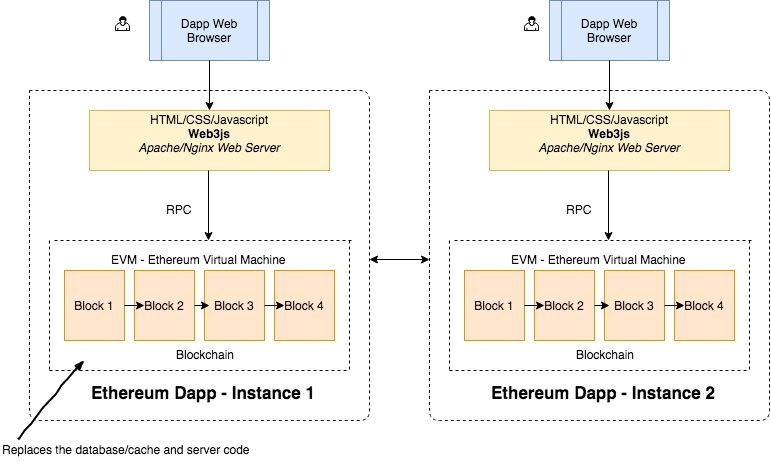
\includegraphics[width=0.6\textwidth, alt={Descrizione dell'architettura di Ethereum}]{immagini/ethereum-architecture.png}
    \caption{Architettura Ethereum} Fonte dell'immagine: \cite{site:etharchitecture}\label{fig:eth-architecture}
\end{figure}

\newpage
Complessivamente, l'applicazione avrà graficamente l'architettura visibile in figura \ref{fig:architettura}, dove viene descritta la composizione del contratto 
e la sua interazione con la parte front-end dell'applicazione, interagendo con la blockchain di test tramite Hardhat.
\begin{figure}[h]
    \centering
    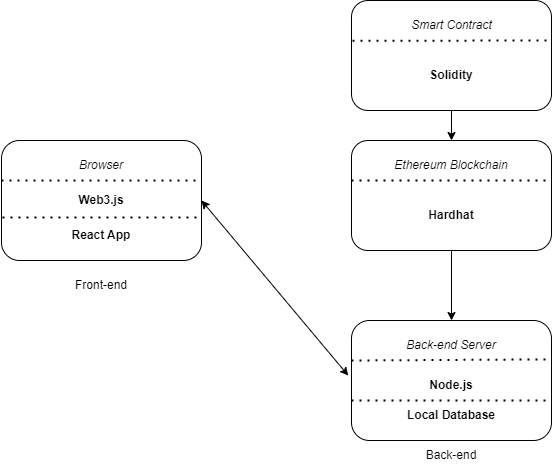
\includegraphics[width=0.6\textwidth, alt={Descrizione dell'architettura dell'applicazione}]{immagini/architettura.png}
    \caption{Architettura applicazione} \label{fig:architettura}
\end{figure}

\section{Codifica}\label{sec:codifica-requisiti}

In questa sezione la descrizione della codifica è suddivisa in due parti, una per la parte back-end e una per la parte front-end.
Si è scelta questa suddivisione per permettere di comprendere subito il contratto libreria utilizzato e le sue funzionalità,
al fine di poter avere una comprensione più chiara della parte front-end, che si basa su di esso per poter implementare quanto previsto in precedenza.

\subsection{Codifica back-end}
Il contratto che viene utilizzato come libreria è parte di un'implementazione della tecnologia \glsfirstoccur{\gls{ssig}} descritta opportunamente nella
sezione \ref{sec:self-sovereign-identity}. Esso offre funzionalità avanzate che consentono la creazione e la gestione di documenti di identità
unici per ciascun utente, associando a ciascuno un \glsfirstoccur{\gls{didg}} considerato univoco.
Globalmente, il contratto definisce le seguenti strutture dati:
\begin{itemize}
    \item \textbf{Parent}, che rappresenta il collegamento gerarchico tra i documenti di identità rilasciato, associando un identificativo al genitore,
    un campo di conferma validità ed una firma;
    \item \textbf{VerificationMethod}, che rappresenta il metodo di verifica associato al documento di identità, comprensivo di un indice, un identificativo,
    un metodo di verifica di firma digitale, un controllore, un identificativo della blockchain associata e un indirizzo dell'account associato a blockchain da verificare;
    \item \textbf{Service}, che rappresenta il servizio associato al documento di identità, comprensivo di un identificativo, un tipo di servizio e il suo indirizzo \textit{URL};
    \item \textbf{DidDocumentData}, che rappresenta i metadati associati ad uno specifico documento di identità, con un suo identificativo, la sua prova di validità, tre mappe per i tipi di autenticazione, deleghe di capacità
    e servizi dei documenti ad essi associati e un e un \textit{Parent}e. Ciò risulta utile nella verifica della catena di fiducia implementata successivamente;
    \item \textbf{DidDocument}, che rappresenta il documento di identità associato all'utente e comprende un identificativo, un metodo di verifica, una delegazione di capacità, un servizio e un \textit{Parent};
    \item \textbf{ResolutionResult}, che rappresenta il risultato della risoluzione del documento di identità, comprendente un identificativo il documento di tipo \textit{DidDocument} associato;
    \item \textbf{ChainResolutionResult}, un vettore di stringhe che racchiude i risultati della risoluzione dei vari documenti di identità associati.
\end{itemize}

Il contratto prevede una serie di metodi, ciascuno con un suo scopo, da me successivamente utilizzati nella parte front-end dell'applicazione.
Ogni metodo descritto è stato utilizzato all'interno di una pagina o componente a seconda dello scopo voluto; globalmente, possiamo specificare:
\begin{itemize}
    \item \textbf{createDid}, che permette la creazione di un documento di identità, associando un \textit{DID} univoco all'utente che ha effettuato la transazione e ritorna il \textit{DID} del nuovo utente aggiunto;
    \item \textbf{createChildTrustedDid}, in grado di creare un nuovo \textit{DID Document} che afferma la delegazione di fiducia dall'utente certificatore (cosiddetto \textit{certification autority}) all'utente con il \textit{DID} specificato.
    Questo permette di creare la catena degli \textit{issuer} fidati, partendo dalla detta \textit{certification autority} e arrivando fino all'utente che ha effettuato la transazione, verificando i suoi dati in modo sicuro.
    Esso prende come parametri l'indirizzo dell'utente a cui delegare la fiducia e la firma della \textit{certification autority};
    \item \textbf{initializeDidDocument}, richiamato dal metodo \textit{createDid}, che inizializza il documento di identità associato all'utente, prendendo come parametri il \textit{DID} dell'utente e il suo indirizzo;
    \item \textbf{addCapabilityDelegation}, che permette di aggiungere una delega di capacità al documento di identità, prendendo come parametro l'indirizzo dell'utente che autenticherà la transazione;
    \item \textbf{addService}, che permette di aggiungere un servizio al documento di identità, prendendo come parametri, l'identificativo, il tipo di servizio e il suo indirizzo \textit{URL};
    \item \textbf{deactivate}, il quale disattiva il \textit{DID Document} associato all'utente che ha effettuato la transazione;
    \item \textbf{resolve}, che ritorna il \textit{DID Document} associato all'utente secondo un determinato \textit{DID} passato come parametro;
    \item \textbf{resolveChain}, che ritorna la catena di fiducia percorsa avendo come ultimo nodo l'utente con il \textit{DID} specificato e ritorna la lista di utenti certificatori a cui si è passati per arrivare all'utente finale;
    \item \textbf{getAuthentication}, per ottenere il metodo di autenticazione associato al documento di identità e provare per certo l'utente abbia acceduto secondo il metodo corretto.
\end{itemize}

\newpage
\subsection{Codifica front-end} \label{sec:codifica-front-end}

\subsubsection{Pagine realizzate}

\paragraph{Home Page}

La pagina definita in codice come \textit{HomePage} è la prima schermata visibile collegandosi al sito, come visibile in figura \ref{fig:pagina-principale}. Essa permette di accedere alle funzionalità principali dell'applicazione.
In particolare, è possibile accedere alla pagina di registrazione e alla pagina di login attraverso l'utilizzo degli appositi componenti.
Essa utilizza i componenti principali di navigazione (nello specifico \textit{Footer} e \textit{NavBar} per gestire le opzioni 
previste per gli utenti a seconda che siano o meno autenticati). L'intera applicazione è infatti racchiusa nel componente \textit{AuthContext}, che permette di gestire lo stato di autenticazione dell'utente.
Per questa, come le altre pagine, ove non diversamente specificato, è prevista l'esportazione di default come funzione \textit{TypeScript}, includendo i componenti utili ove previsto e 
separando la struttura impostata in \textit{HTML} e la presentazione impostata in \textit{CSS} da file omonimo, presente nella stessa cartella della pagina.

\begin{figure}[h]
    \centering
    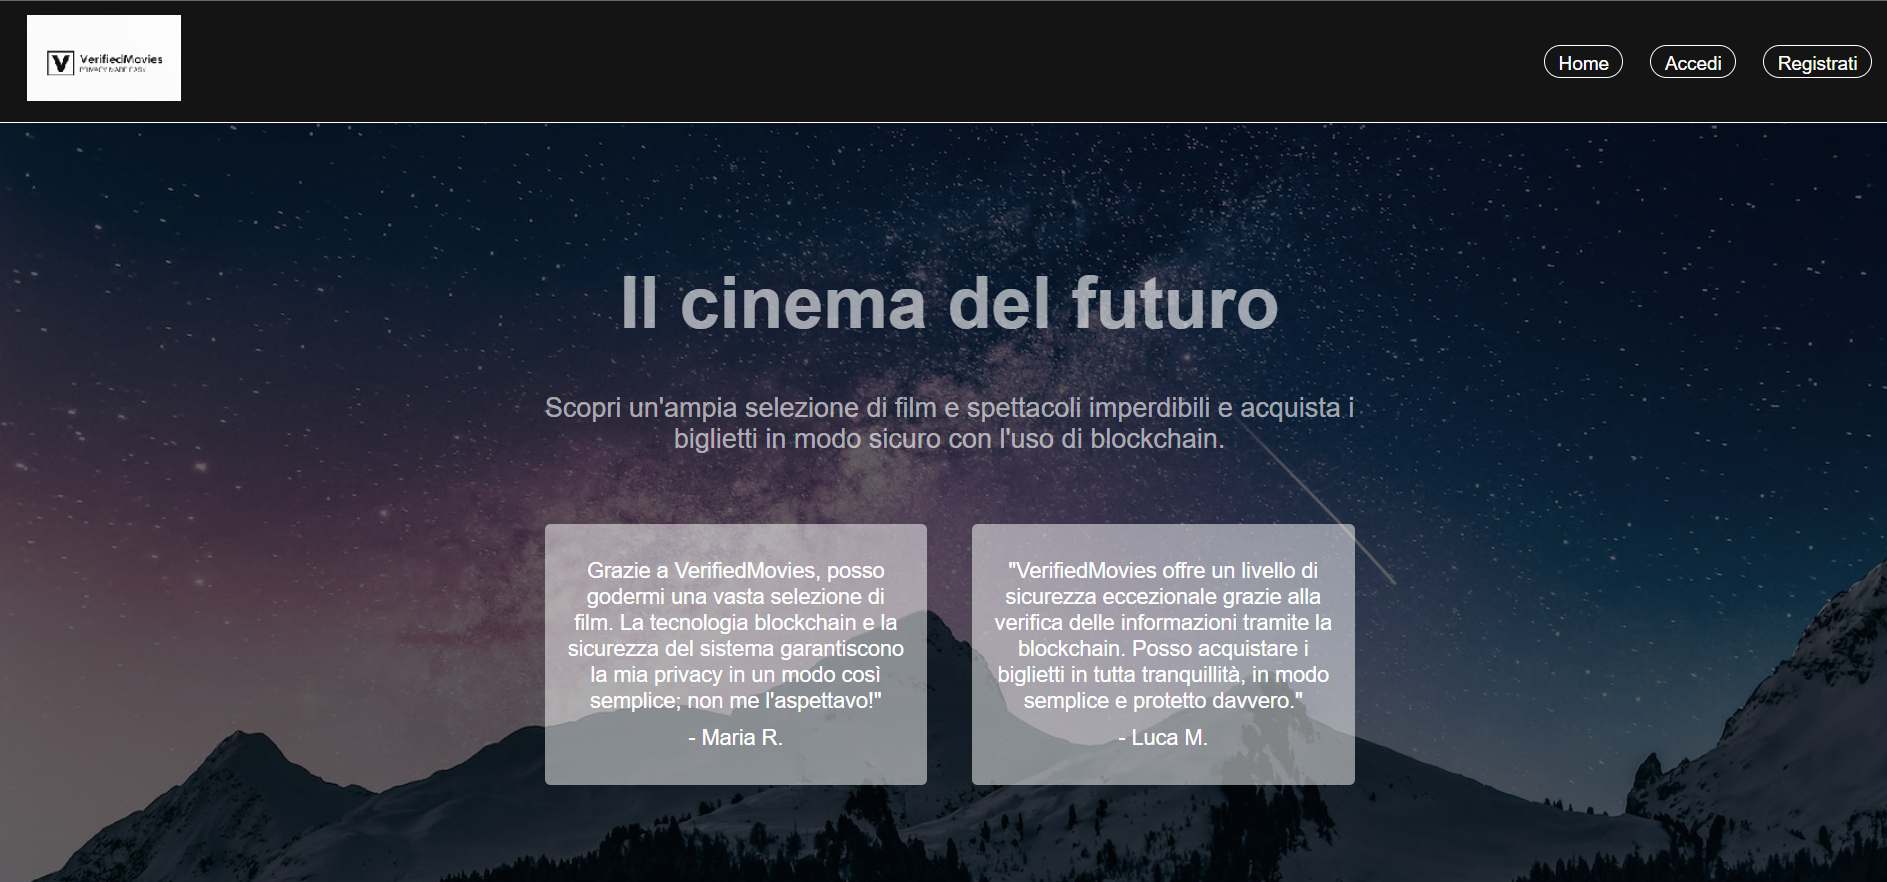
\includegraphics[width=0.6\textwidth, alt={Pagina principale dell'applicazione}]{immagini/frontend/home.png}
    \caption{Pagina principale}\label{fig:pagina-principale}
\end{figure}

Si noti l'utilizzo di un'immagine di sfondo senza diritti d'autore, proveniente dal sito \textit{Pexels}, che permette di rendere la pagina più accattivante e di presentare l'idea di un'identità digitale.
Tutto il sito è stato anche sviluppato per consentire una piena navigazione da mobile, come visibile in figura \ref{fig:pagina-principale-mobile}.
Presenta infatti un layout responsive, che si adatta alle dimensioni dello schermo del dispositivo utilizzato, avendo come punto di rottura una dimensione 
di 768 pixel.
\begin{figure}[h]
    \centering
    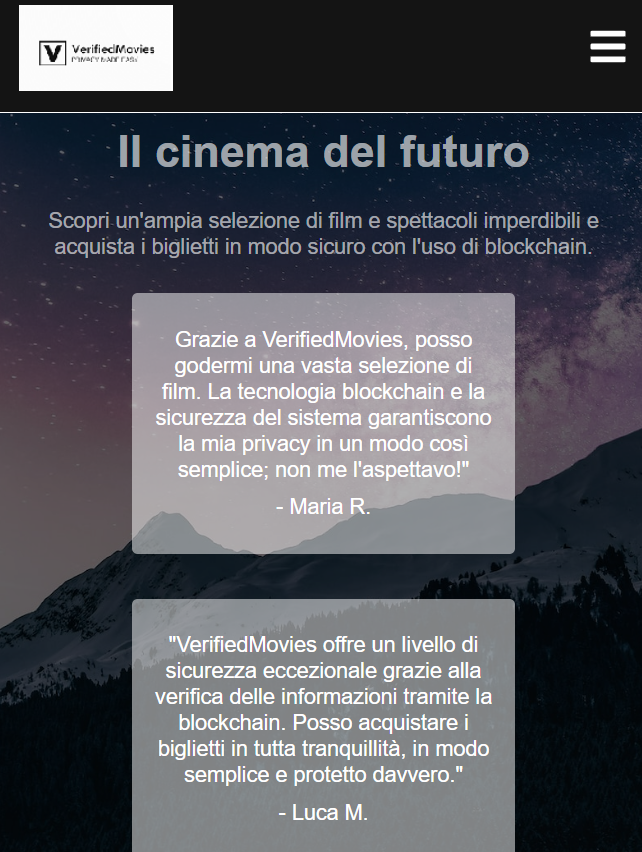
\includegraphics[width=0.3\textwidth, alt={Pagina principale dell'applicazione vista da cellulare}]{immagini/frontend/home-mobile.png}
    \caption{Pagina principale vista da cellulare}\label{fig:pagina-principale-mobile}
\end{figure}

In questa pagina, viene creato il \textit{DID} associato all'utente e la catena di \textit{issuer} di test che permette di verificare la validità del meccanismo di catena di fiducia,
poi spiegato in dettaglio nella pagina dei film dove viene attivato tale meccanismo.

\paragraph{Registrazione}

Nella pagina in oggetto, definita in codice come \textit{RegisterView}, l'utente è portato a registrarsi all'applicazione, inserendo i dati richiesti, come visibile in figura \ref{fig:pagina-registrazione}.
Come descritto dai casi d'uso, vi è un controllo sulla validità dei dati inseriti, verificando se \textit{DID} o la email inserita siano già esistenti.
Questa è la prima che utilizza lo smart contract libreria direttamente; viene infatti implementato un meccanismo di \textit{challenge-response}
per verificare che l'utente sia in possesso del \textit{DID} inserito. Tale meccanismo è stato implementato per non dipendere da piattaforme esterne legate a blockchain
come la nota estensione \textit{MetaMask}, al fine di realizzare un sistema interno che permetta di confermare la validità dei dati dell'utente, sempre usando blockchain,
sia per il meccanismo di login che registrazione, come richiesto dal proponente. 

\begin{figure}[h]
    \centering
    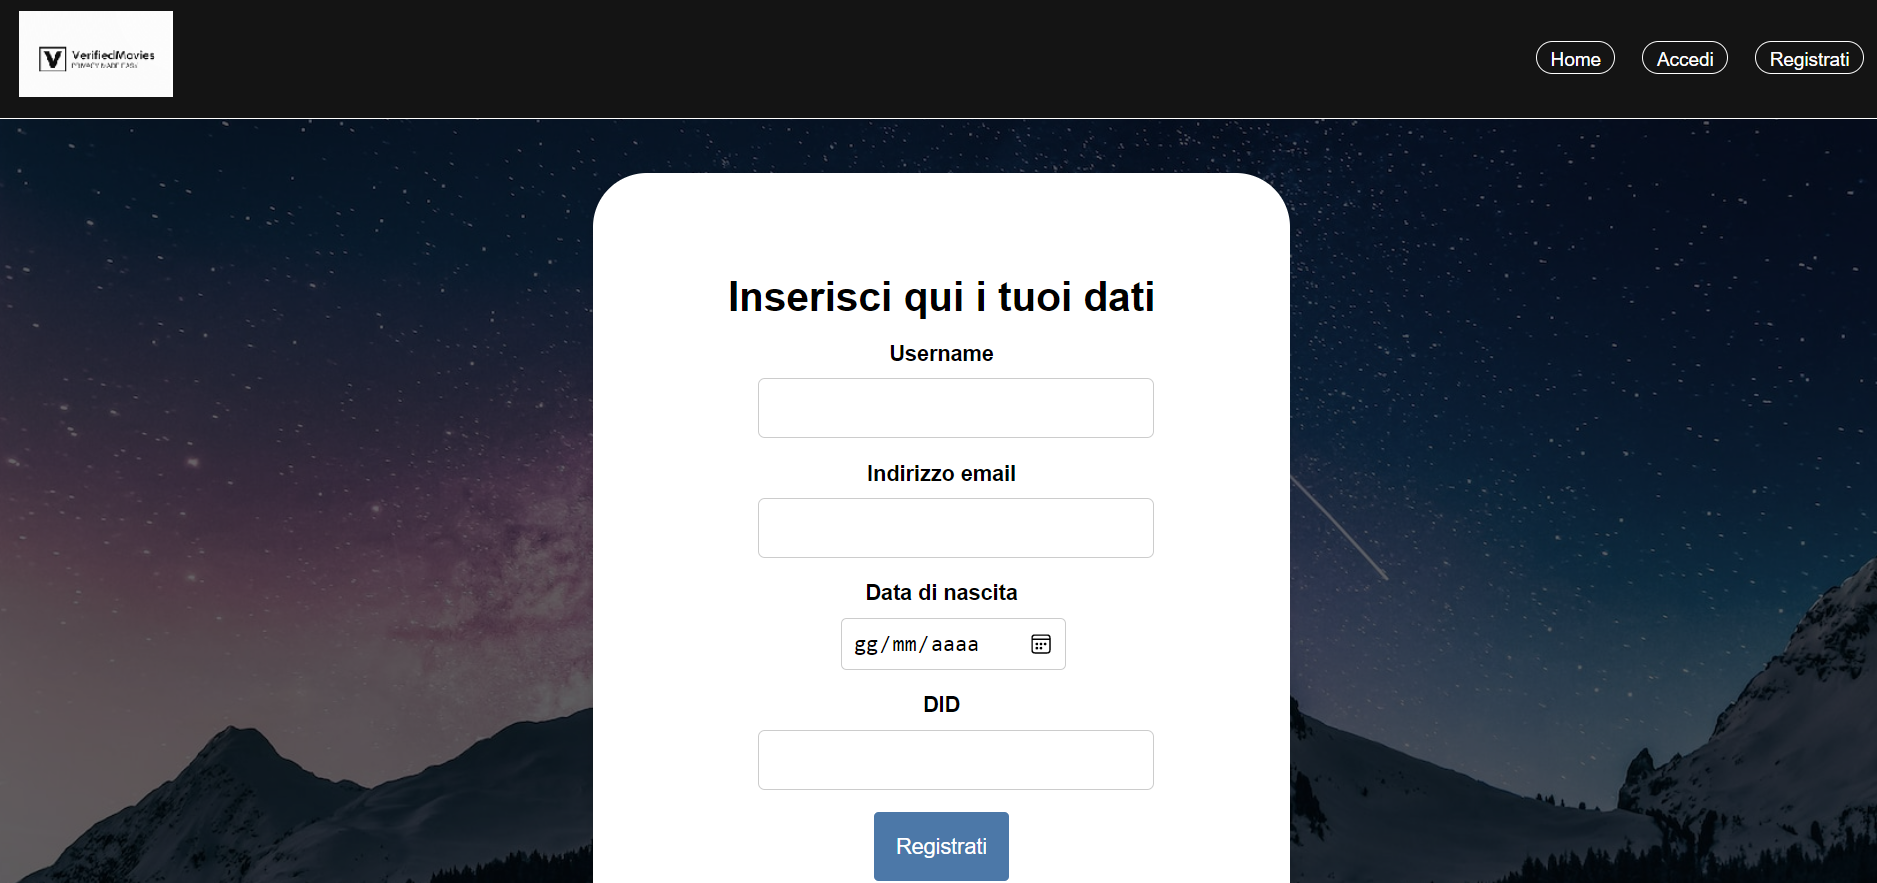
\includegraphics[width=0.6\textwidth, alt={Pagina principale dell'applicazione}]{immagini/frontend/register.png}
    \caption{Pagina principale} \label{fig:pagina-registrazione}
\end{figure}

Si prevede, come visibile in figura \ref{fig:sfida}, che l'utente cifri con la propria chiave privata un numero presentato a schermo;
in questa fase viene generata una prova di autenticazione in formato \textit{JSON}, che dimostra che l'utente vuole autenticarsi con il suo \textit{DID} avendo firmato il numero
e chiamando il metodo \textit{getAuthentication} dello smart contract.
Se la firma digitale corrisponde e il \textit{DID} corrisponde a quello creato inizialmente, allora la verifica passa e la registrazione è confermata con successo, 
avvisando l'utente con un messaggio apposito. 

\begin{figure}[h]
    \centering
    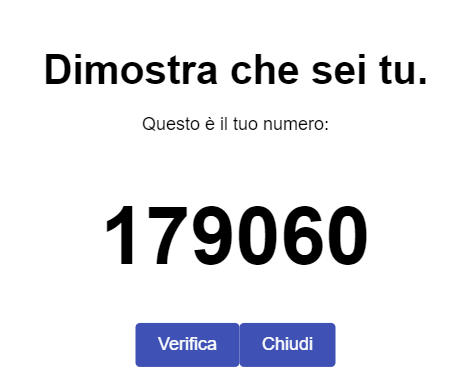
\includegraphics[width=0.3\textwidth, alt={Meccanismo di sfida per conferma dell'identità dell'utente}]{immagini/frontend/challenge-response.png}
    \caption{Meccanismo di conferma identità dell'utente} \label{fig:sfida}
\end{figure}

\newpage
\paragraph{Login}
Nella pagina, definita in codice come \textit{LoginView}, è presente un modulo di inserimento dei dati di accesso, come visibile in figura \ref{fig:pagina-login}.
Al fine di minimizzare i dati raccolti, l'utente dovrà inserire solo il suo \textit{DID}, come previsto dai casi d'uso, 
in quanto i dati inseriti nella fase di registrazione sono inseriti ed associati all'interno del documento presentato per l'accesso.
Anche in questo caso, come per la registrazione, è previsto un controllo sulla validità dei dati inseriti, verificando se il \textit{DID} inserito sia già esistente.
In base alle specifiche dette, è previsto lo stesso meccanismo di \textit{challenge-response} dettagliato nel paragrafo precedente da figura \ref{fig:sfida}
per verificare la validità dei dati inseriti.

\begin{figure}[h]
    \centering
    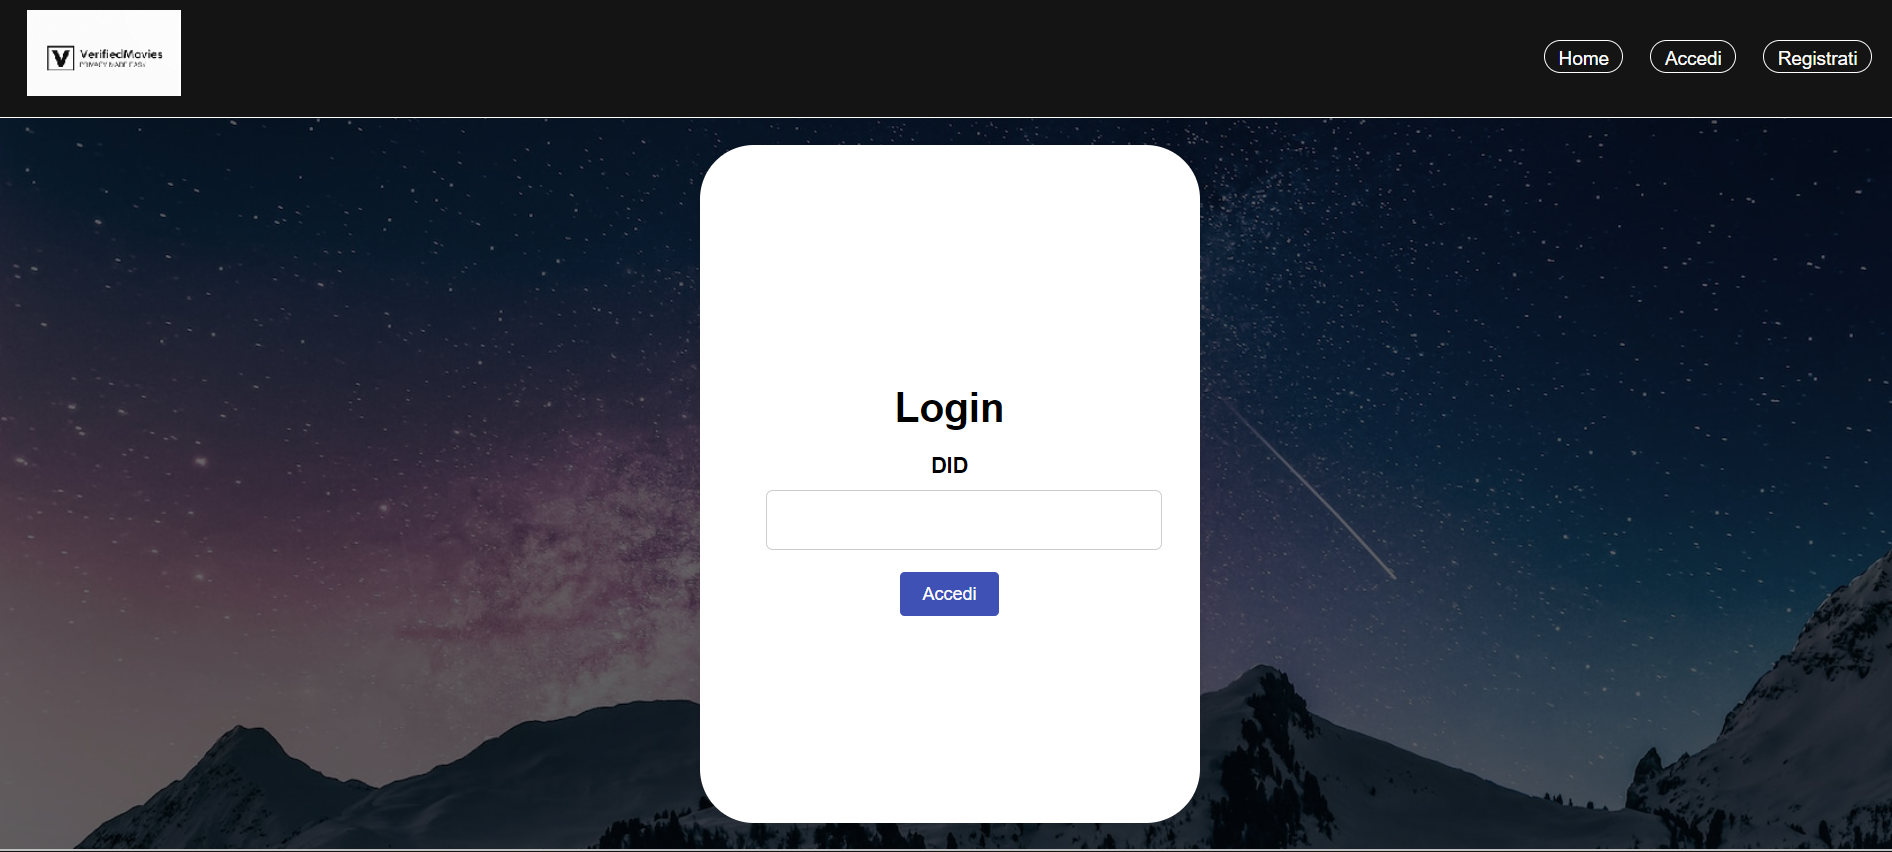
\includegraphics[width=0.6\textwidth, alt={Pagina di accesso all'applicazione}]{immagini/frontend/login.png}
    \caption{Pagina di login}\label{fig:pagina-login}
\end{figure}

\paragraph{Film}

In questa pagina, definita in codice come \textit{MoviesView} sono presenti i film disponibili all'interno del sistema, come visibile in figura \ref{fig:pagina-film}.
Come visibile, in questo caso, le opzioni di navigazione previste per l'utente cambiano, mostrando la pagina in oggetto, al link \textit{/Film},
e le successive pagine di questa sezione, comprendente la pagina di gestione del profilo, di visualizzazione delle prenotazioni presenti e il link per effettuare il logout.
Per ogni film è presente un'immagine, il titolo, la descrizione, una categoria e una valutazione in termini di età.
É inoltre presente il componente \textit{SearchBox} che permette di filtrare i film in base al titolo.
\begin{figure}[h]
    \centering
    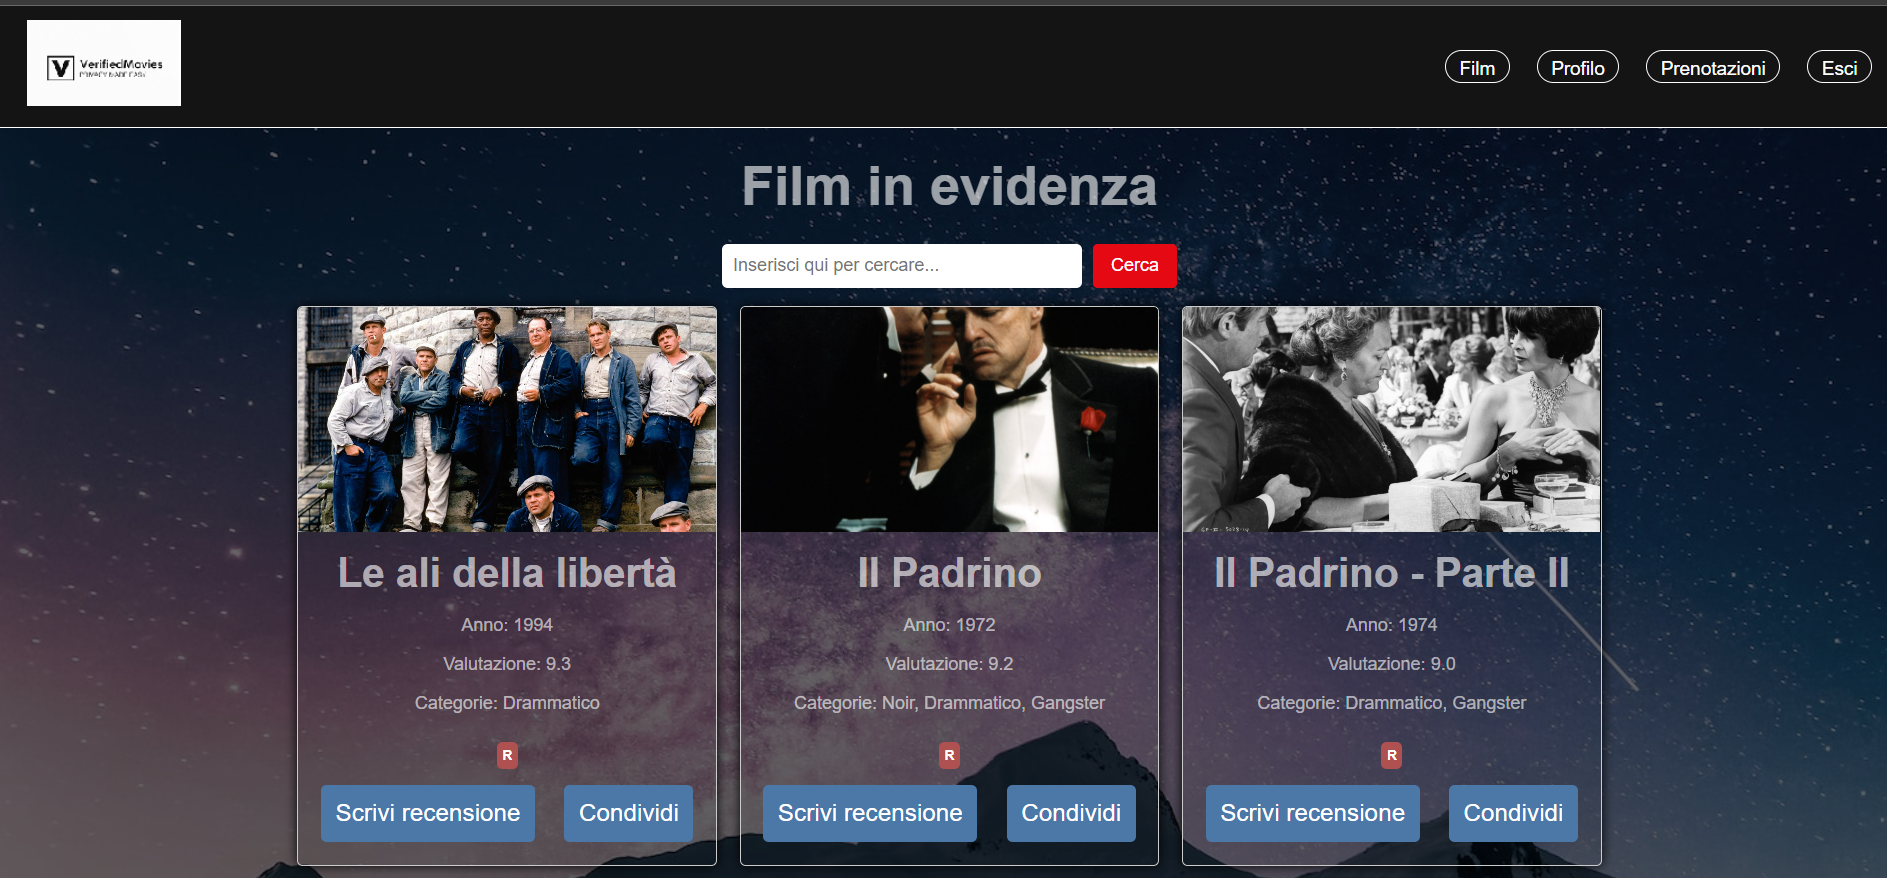
\includegraphics[width=0.6\textwidth, alt={Pagina contenente i film dell'applicazione}]{immagini/frontend/movies.png}
    \caption{Pagina dei film dell'applicazione}\label{fig:pagina-film}
\end{figure}

Ogni film permette la sua prenotazione cliccando sopra l'elemento grafico visualizzato; ogni film soggetto a limite d'età rispetto all'età
calcolata dalla data di nascita dell'utente, innesca il meccanismo di verifica dell'età su cui si basa l'intera applicazione, visibile graficamente
in figura \ref{fig:verifica-eta}.
Come per la pagina home, le immagini presenti sono state prese dal noto portale di film \textit{IMDB}, utilizzate per fini puramente dimostrativi e non commerciali.

\begin{figure}[h]
    \centering
    
\includegraphics[width=0.6\textwidth, alt={Finestra visualizzata di verifica dell'età}]{immagini/frontend/age-verification.png}
    \caption{Finestra di verifica dell'età}\label{fig:verifica-eta}
\end{figure}

Il meccanismo prevede l'utilizzo di specifici tipi \textit{TypeScript} che permettono di definire il tipo di \textit{Verifiable Credential} e \textit{Verifiable Presentation}
utilizzati, secondo la definizione presente in sezione \ref{sec:analisi-sistema} coerente agli standard.
L'implementazione realizzata prevede come primo passaggio una funzione di creazione della \textit{Verifiable Credential} che genera una firma digitale secondo lo standard \textit{CLSignature2019}, con le specifiche seguenti:
\begin{itemize}
    \item l'utilizzo della chiave privata dell'\textit{issuer}, usato per firmare la credenziale;
    \item l'utilizzo della chiave pubblica, usata per verificare la firma;
    \item la generazione di un numero casuale, usato per creare la prova di correttezza della firma;
    \item la generazione di un valore di firma, usato per creare la prova di correttezza della firma;
    \item la generazione di una prova di correttezza della firma, usato per verificare la validità della firma.
\end{itemize}
Questo tipo di firma viene utilizzato in quanto permette di realizzare il meccanismo \glsfirstoccur{\gls{zkpg}} (basandomi sulla standardizzazione in \cite{site:zkpstandard}); infatti, i dati dell'utente vengono creati ed incapsulati
all'interno di uno schema di appartenenza comune. La verifica della firma permette di certificare che l'utente sia in possesso di una credenziale valida, senza rivelare
i dati contenuti al suo interno. 
Inoltre, secondo il meccanismo di \glsfirstoccur{\gls{ssig}}, occorre fare riferimento a tre soggetti in questo sistema:
\begin{itemize}
    \item l'\textit{issuer}, che crea la credenziale e la firma. Questo viene generato in fase di accesso al sito;
    \item l'\textit{holder}, che possiede la credenziale ed è l'utente in possesso del suo \textit{DID};
    \item il \textit{verifier}, che verifica la validità della credenziale e ne estrae i dati. In questo caso è il sito stesso del cinema che verifica la validità della credenziale.
\end{itemize}

Le specifiche del flusso logico seguito fanno riferimento a in \cite{site:clsignature2}.

La credenziale creata internamente ha il seguente aspetto:
\begin{lstlisting}[language=json]
    const vc: VCDIVerifiableCredential = {
        '@context': ['https://www.w3.org/2018/credentials/v1'],
        id: 'http://localhost:3000/ageCredentialSchema',
        type: ['VerifiableCredential'],
        credentialSchema: { 
            id: userDid ? userDid : "",
            type: "VerifiableCredential"
        },        
        issuer: {
          id: issuerDid,
          publicKey: publicKeyHex 
        } as IssuerObject,
        issuanceDate: new Date().toISOString(),
        credentialSubject: {
          id: userDid,
          age: userData.age,
          type: 'VerifiableCredential',
        } as CredentialSubject,
        proof: {
          type: "CLSignature2019", 
          issuerData: issuerDid, 
          attributes: masterSecret,
          signature: signature,
          signatureCorrectnessProof: proof.signatureCorrectnessProof,
        },
      };
\end{lstlisting}
L'utilizzo di questo tipo di firma digitale è usata in soluzioni blockchain di secondo livello, come \textit{Hyperledger Indy}, 
secondo le specifiche dettagliate in \cite{site:clsignature}. \\

Successivamente, viene utilizzata una funzione che prevede la creazione di una \textit{Verifiable Presentation} che contiene la \textit{Verifiable Credential} creata precedentemente,
e avendo come parametri al firma e la prova di correttezza generata prima. L'implementazione adatta flessibilmente i campi di verifica presenti per il tipo di firma digitale, 
,adattando al tipo di firma quanto previsto in \cite{site:vpw3c}, diventando come segue:
\begin{lstlisting}[language=json]
    const vp: VerifiablePresentation = {
        '@context': [
          "https://www.w3.org/2018/credentials/v1",
          "https://www.w3.org/2018/credentials/examples/v1"
        ],
        type: "VerifiablePresentation",
        verifiableCredential: [vc],
        proof: {
          type: "CLSignature2019",
          proofValue: {
            signatureValue: {
              r: signature.r.toString(16),
              s: signature.s.toString(16),
            },
            signatureCorrectnessProof: signatureCorrectnessProof,
          },
        }
      };
\end{lstlisting}

Nella successiva fase, viene verificata la firma digitale immessa, utilizzando la chiave pubblica dell'\textit{issuer}, e la prova di correttezza generata precedentemente.
Tale passaggio prevede l'utilizzo di una funzione che utilizza il calcolo della curva ellittica \textit{secp256k1}, usato all'interno della piattaforma Bitcoin, per verificare all'interno di blockchain
la validità delle transazioni trasmesse. Questa si compone di vari passaggi:
\begin{itemize}
    \item generazione della coppia di chiavi, pubblica e privata, generando un valore casuale intero definito come \textit{nonce};
    \item generazione di un valore casuale, generando un valore \textit{hash} univoco ai dati trasmessi e una firma, composta da una coppia di valori \textit{r} e \textit{s}, 
    dati dal valore del punto di firma e del valore \textit{nonce} generato precedentemente;
    \item verifica della firma, utilizzando la chiave pubblica, la firma fornita e il valore hash per verificare se la coppia di chiavi iniziale è valida.
\end{itemize}

Come ultimo punto, viene verificata la catena di fiducia della \textit{Verifiable Presentation} creata, utilizzando la chiave pubblica dell'\textit{issuer} e risalendo
la catena di fiducia fino alla radice, verificando la firma digitale di ogni \textit{issuer} creato nella pagina iniziale del sito attraverso le funzioni del contratto libreria
\textit{resolve()} e \textit{resolveChain()}.

Graficamente, ciascuno di questi passaggi simula una fase di caricamento, mostrando all'utente un messaggio e un'icona di caricamento, per indicare che il sistema sta eseguendo
le operazioni fin qui descritte, come visibile in figura \ref{fig:verifica-eta-corso}.

\begin{figure}[h]
    \centering
    
\includegraphics[width=0.6\textwidth, alt={Finestra visualizzata di caricamento durante la verifica dell'età}]{immagini/frontend/verification-doing.png}
    \caption{Esempio di caricamento durante la verifica dell'età}\label{fig:verifica-eta-corso}
\end{figure}

\newpage 

In ultimo, come descritto inizialmente in questo paragrafo, per l'utente è possibile lasciare recensioni e condividere il film in oggetto.
La recensione prevede, a fini dimostrativi, l'inserimento di un testo, salvato convenzionalmente all'interno del portale in locale.
L'inserimento è visibile in figura \ref{fig:recensione-film}.

\begin{figure}[h]
    \centering
    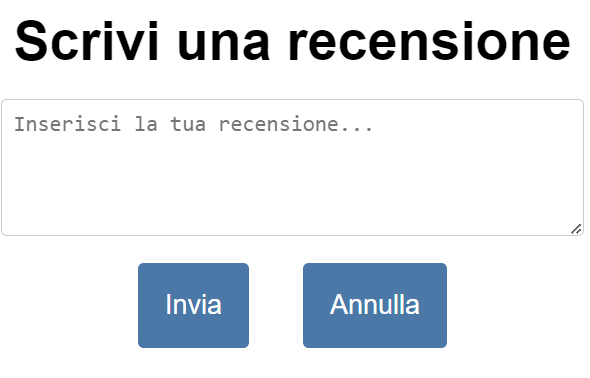
\includegraphics[width=0.3\textwidth, alt={Schermata di inserimento di una recensione per un film}]{immagini/frontend/review.png}
    \caption{Recensione per un film}\label{fig:recensione-film}
\end{figure}

Infine, la condivisione di un film genera un link con i metadati dello stesso e comprendente il titolo del film come parametro di riconoscimento.
Questa azione è visibile in figura \ref{fig:condivisione-film}.

\begin{figure}[h]
    \centering
    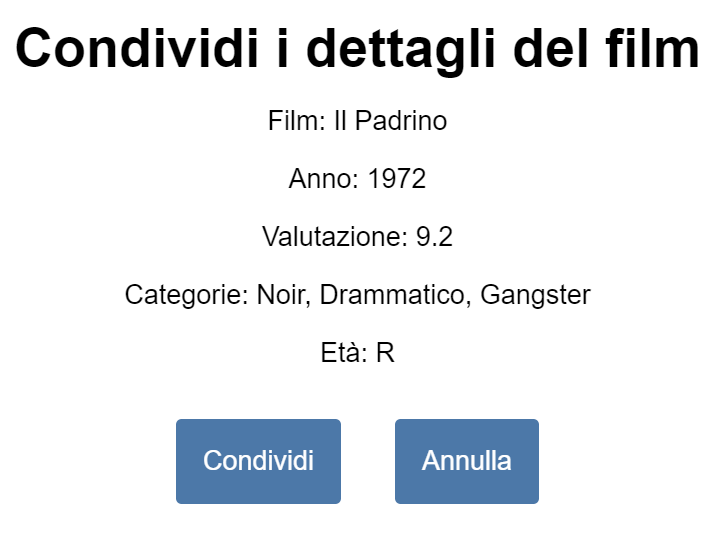
\includegraphics[width=0.3\textwidth, alt={Schermata di condivisione di un film}]{immagini/frontend/share.png}
    \caption{Condivisione di un film}\label{fig:condivisione-film}
\end{figure}

\paragraph{Prenotazione del film}
Per questa pagina, accessibile una volta effettuata la verifica dell'età, viene mostrata una finestra per confermare la prenotazione del film selezionato, 
inserendo il numero di posti desiderati, la data di prenotazione, l'orario e il numero di biglietti tra una serie di opzioni disponibili, come visibile in figura \ref{fig:prenotazione-film}.

\begin{figure}[h]
    \centering
    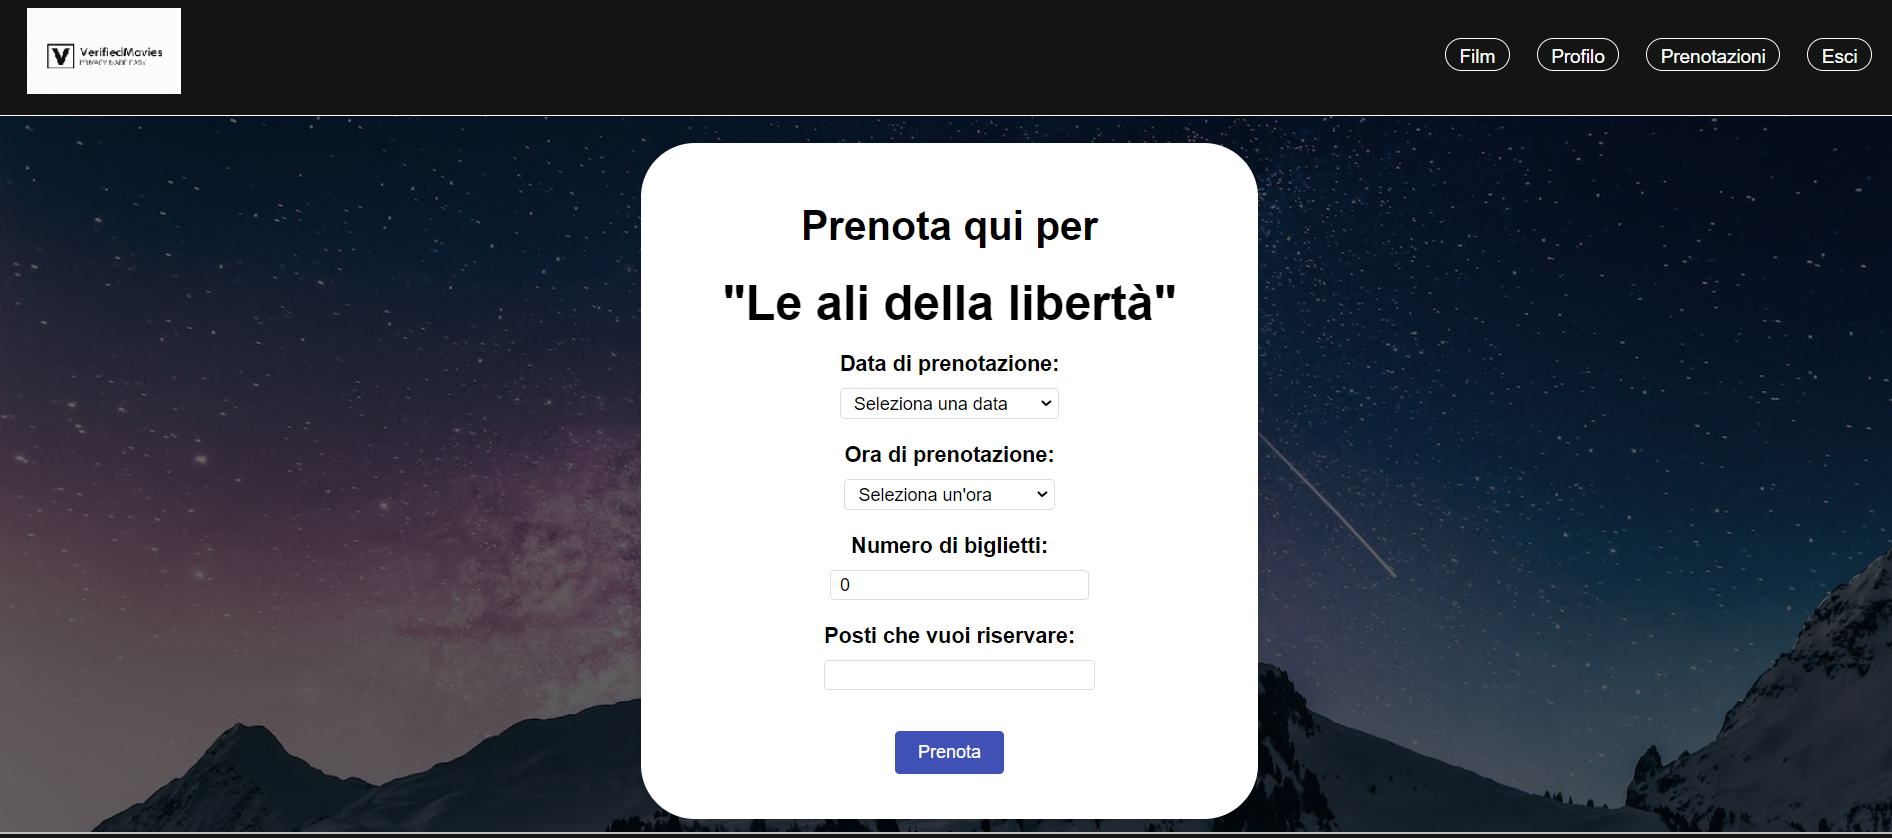
\includegraphics[width=0.6\textwidth, alt={Schermata della pagina di prenotazione del film selezionato}]{immagini/frontend/movie-booking.png}
    \caption{Pagina di prenotazione del film selezionato}\label{fig:prenotazione-film}
\end{figure}

\newpage

Una volta effettuata la prenotazione, viene mostrata una finestra di conferma, come visibile in figura \ref{fig:conferma-prenotazione}.
\begin{figure}[h]
    \centering
    
\includegraphics[width=0.3\textwidth, alt={Schermata della pagina di conferma della prenotazione del film selezionato}]{immagini/frontend/movie-booking-done.png}
    \caption{Finestra di conferma della prenotazione del film selezionato}\label{fig:conferma-prenotazione}
\end{figure}

\paragraph{Lista delle prenotazioni}
Per questa pagina, accessibile una volta effettuata la verifica dell'età e la prenotazione del film, viene mostrata una lista delle prenotazioni effettuate dall'utente.
I dati del film sono salvati e mostrati in seguito uno all'altro, recuperati dal salvataggio in locale all'interno di \textit{localStorage}, come visibile in figura \ref{fig:lista-prenotazioni}.

\begin{figure}[h]
    \centering
    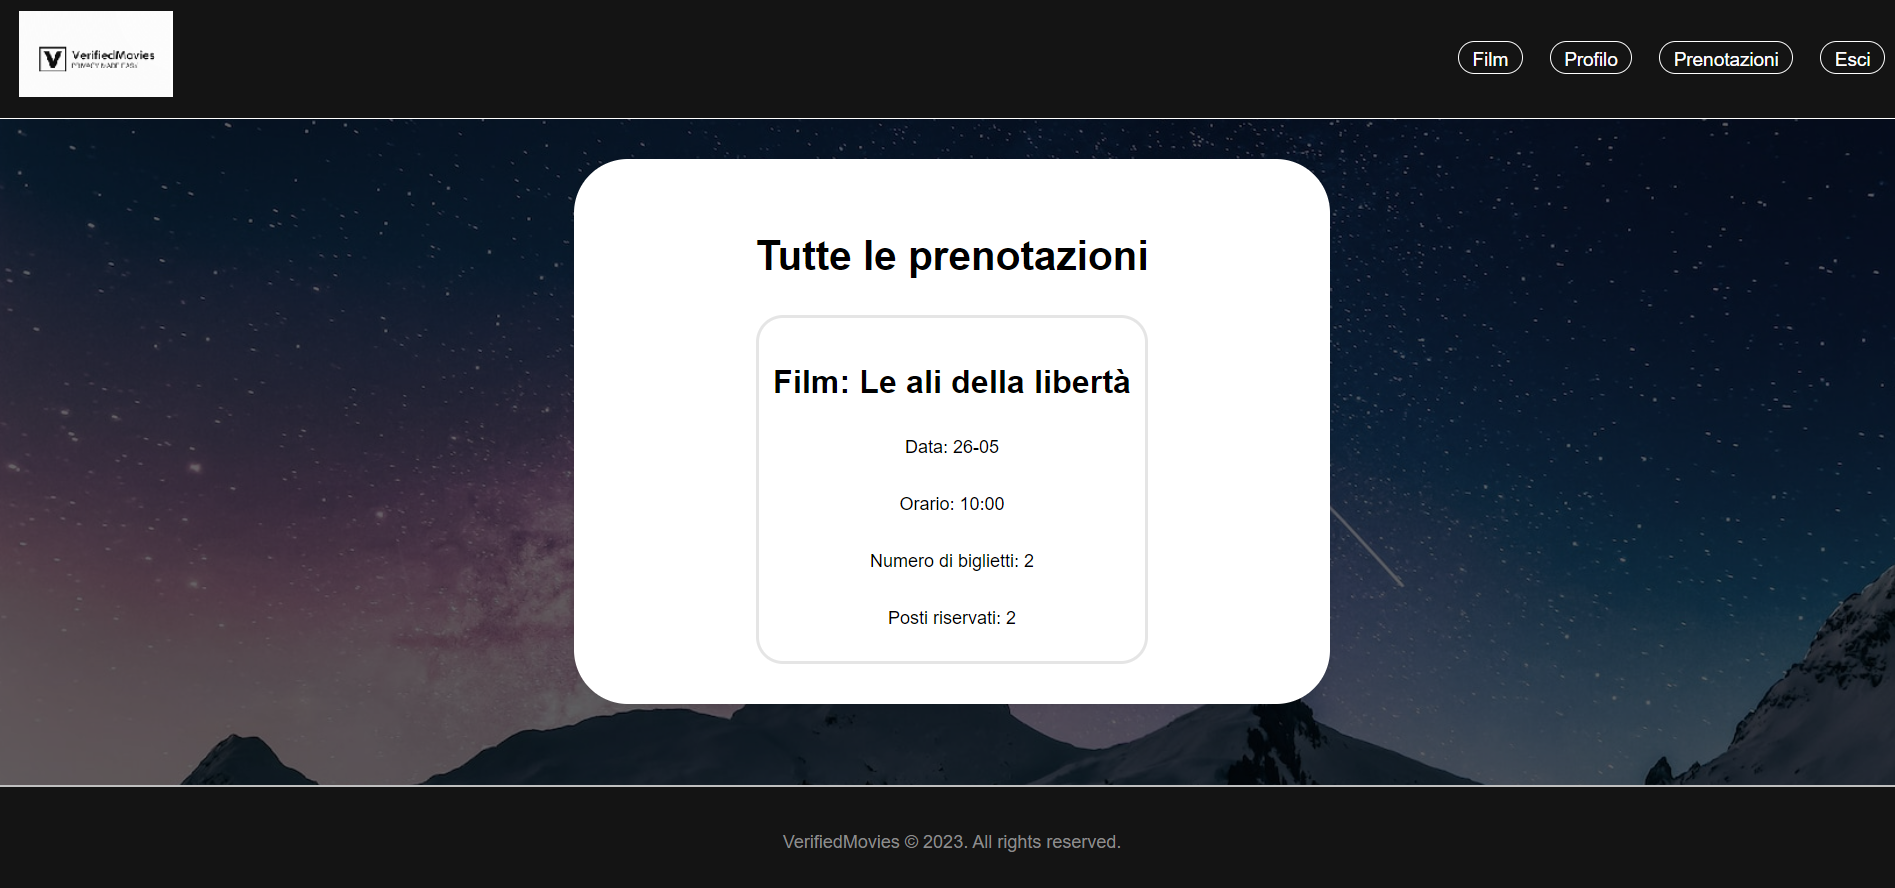
\includegraphics[width=0.6\textwidth, alt={Schermata della pagina di lista delle prenotazioni effettuate}]{immagini/frontend/movie-booking-list.png}
    \caption{Pagina della lista delle prenotazioni effettuate}\label{fig:lista-prenotazioni}
\end{figure}

\newpage
\paragraph{Profilo}

All'interno di questa pagina, viene mostrato un riepilogo dei dati dell'utente, come visibile in figura \ref{fig:profilo}.
Questi dati, salvati sempre in locale all'interno di \textit{localStorage}, sono recuperati e mostrati all'utente, visibili nella pagina.
Per evitare che i dati dell'utente siano modificati da terzi in modo malevolo, sono state implementate due funzioni di cifratura e decifratura 
dei dati secondo una funzione \textit{TypeScript} adattando l'algoritmo di cifratura \textit{AES}, utilizzando come chiave di cifratura il \textit{DID} dell'utente.
In questa funzione, i dati vengono suddivisi in blocchi di dimensioni fisse, effettuando poi un'operazione di \textit{XOR} con un valore casuale e crittografando i dati in successione.
Questi dati sono crittografati in formato numerico, successivamente decrittati utilizzando la stessa chiave utilizzata in precedenza.
La pagina offre la possibilità di modificare i propri dati oppure cancellare il proprio profilo, chiamando il metodo dello smart contract \textit{deactivate()}
che permette di disattivare il \textit{DID} associato all'utente, cancellando poi i suoi dati in modo corretto.
\begin{figure}[h]
    \centering
    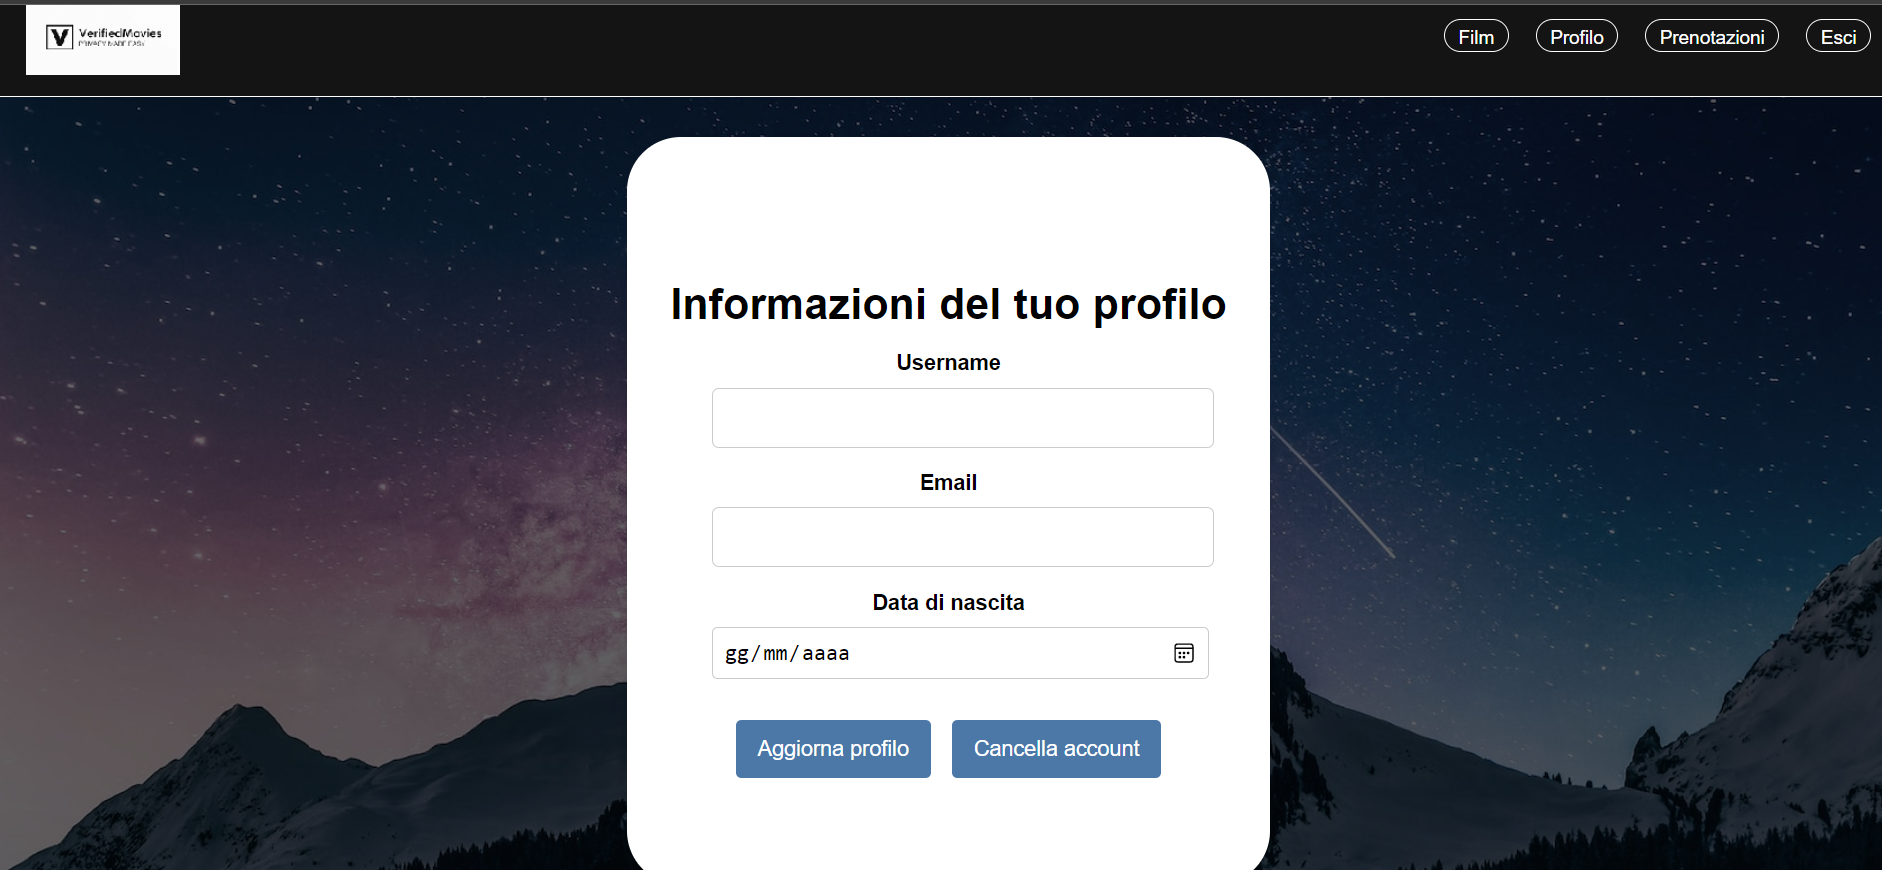
\includegraphics[width=0.6\textwidth, alt={Schermata della pagina di gestione del profilo dell'utente}]{immagini/frontend/account.png}
    \caption{Pagina di gestione dei dati dell'utente}\label{fig:profilo}
\end{figure}

\paragraph{Errore 404}

Se l'utente inserisse un URL non valido, verrà mostrata una pagina di errore 404, come visibile in figura \ref{fig:errore-404}.
Questa contiene un link che reindirizza l'utente alla pagina principale del portale.

\begin{figure}[h]
    \centering
    
\includegraphics[width=0.6\textwidth, alt={Schermata della pagina di errore 404}]{immagini/frontend/404.png}
    \caption{Pagina di errore 404}\label{fig:errore-404}
\end{figure}

\newpage

\subsubsection{Componenti realizzati}

\paragraph{AuthContext}
Il componente è stato realizzato per gestire l'autenticazione in tutta l'applicazione; infatti, viene utilizzato per salvare lo stato dell'utente,
permettendo di incapsulare la logica di autenticazione e di renderla disponibile in tutti i componenti dell'applicazione.
In questo modo, è possibile discriminare quali voci di menu visualizzare in base all'utente e se un determinato utente può accedere ad una determinata pagina.
La navigazione è permessa tramite l'utilizzo della libreria \textit{react-router-dom}, che permette di definire delle rotte e di reindirizzare l'utente in base alla rotta richiesta.
Ciascun componente, da qui in avanti, prevede, come descritto per le pagine, l'esportazione di default come funzione \textit{TypeScript}, includendo la sua struttura impostata in \textit{HTML} e la presentazione impostata in \textit{CSS} da file omonimo
e presente nella stessa cartella del componente.

\paragraph{Footer}
Il componente è stato realizzato per gestire il footer dell'applicazione, che viene visualizzato in tutte le pagine dell'applicazione.
Il footer contiene i principali dati di navigazione del sito e contiene un link che permette di ritornare su nella pagina corrente, nascosto a livello visivo, ma accessibile tramite \textit{screen reader}.

\paragraph{NavBar}
Il componente è stato realizzato per gestire la barra di navigazione dell'applicazione, che viene visualizzata in tutte le pagine dell'applicazione; in questo caso, se l'utente è autenticato vengono
mostrati i collegamenti relativi alla pagina principale, al login e alla registrazione, altrimenti vengono visualizzate le voci di menu relative alla pagina principale, alla pagina dei film, al profilo e alla lista di prenotazioni effettuate.
Per poter effettuare correttamente il logout e riconoscere l'utente, è stato necessario utilizzare la funzione \textit{useContext} di \textit{React}, utilizzando degli \textit{hooks} personalizzati per
gestire la presentazione e i propri link di navigazione.

\paragraph{PrivateRoute}

Questo componente è stato realizzato per gestire le rotte protette dell'applicazione, che vengono utilizzate per accedere alle pagine di prenotazione e di lista delle prenotazioni.
Nel caso in cui l'utente non sia autenticato e voglia accedere ad uno dei link protetti, per semplicità a fini applicativi,
l'utente viene reindirizzato automaticamente alla pagina di login. Di fatto, gestisce con la funzione di autenticazione gli elementi presenti e rileva,
in base al contesto, se l'utente sia autenticato o meno, reindirizzandolo alla pagina di login o alla pagina richiesta.

\paragraph{ScreenReaderHelp}

Il componente è stato progettato e sviluppato con l'obiettivo di fornire un supporto agli screen reader all'interno dell'applicazione. 
Esso è stato creato per garantire che i contenuti presenti sulla pagina siano accessibili agli utenti che utilizzano screen reader per navigare e comprendere il contenuto.
Tramite il suo stile, è possibile nasconderne il contenuto visivamente, assicurandosi che sia accessibile solo agli screen reader.

\paragraph{SearchBox}

Il componente è stato realizzato per gestire la barra di ricerca dei film, che viene visualizzata nella pagina dei film.
La ricerca viene effettuata in base al titolo dello stesso e, a fini di estensibilità, è possibile aggiungere altri parametri di ricerca, previsti per il tipo interno \textit{Movie}
con le caratteristiche descritte nella pagina di visualizzazione dei film presenti.
La funzionalità di ricerca è resa possibile grazie all'uso di un semplice \textit{hook}, che permette di gestire lo stato della ricerca e di aggiornarlo in base al testo inserito dall'utente.

\paragraph{Notification}

Tale componente è stato realizzato per gestire la visualizzazione degli errori e dei relativi messaggi nelle varie situazioni, come ad esempio la registrazione di un utente già esistente
oppure la mancata compilazione di campi all'interno dei moduli del sito. In questo caso, viene utilizzato un \textit{hook} per gestire lo stato della notifica e per aggiornarlo in base al messaggio
di errore ricevuto, mostrando poi il messaggio all'utente.